\documentclass{article}

\usepackage{graphicx}
\usepackage{tikz}
\usepackage{tikzsymbols}
\usetikzlibrary{calc,patterns,shapes.geometric}
\pagestyle{empty}
\usepackage[margin=0pt]{geometry}
\geometry{papersize={14in,12in}}

\def\centerarc[#1](#2)(#3:#4:#5){\draw[#1] ($(#2)+({#5*cos(#3)},{#5*sin(#3)})$) arc (#3:#4:#5);}

\begin{document}
	\begin{figure}
		\centering
		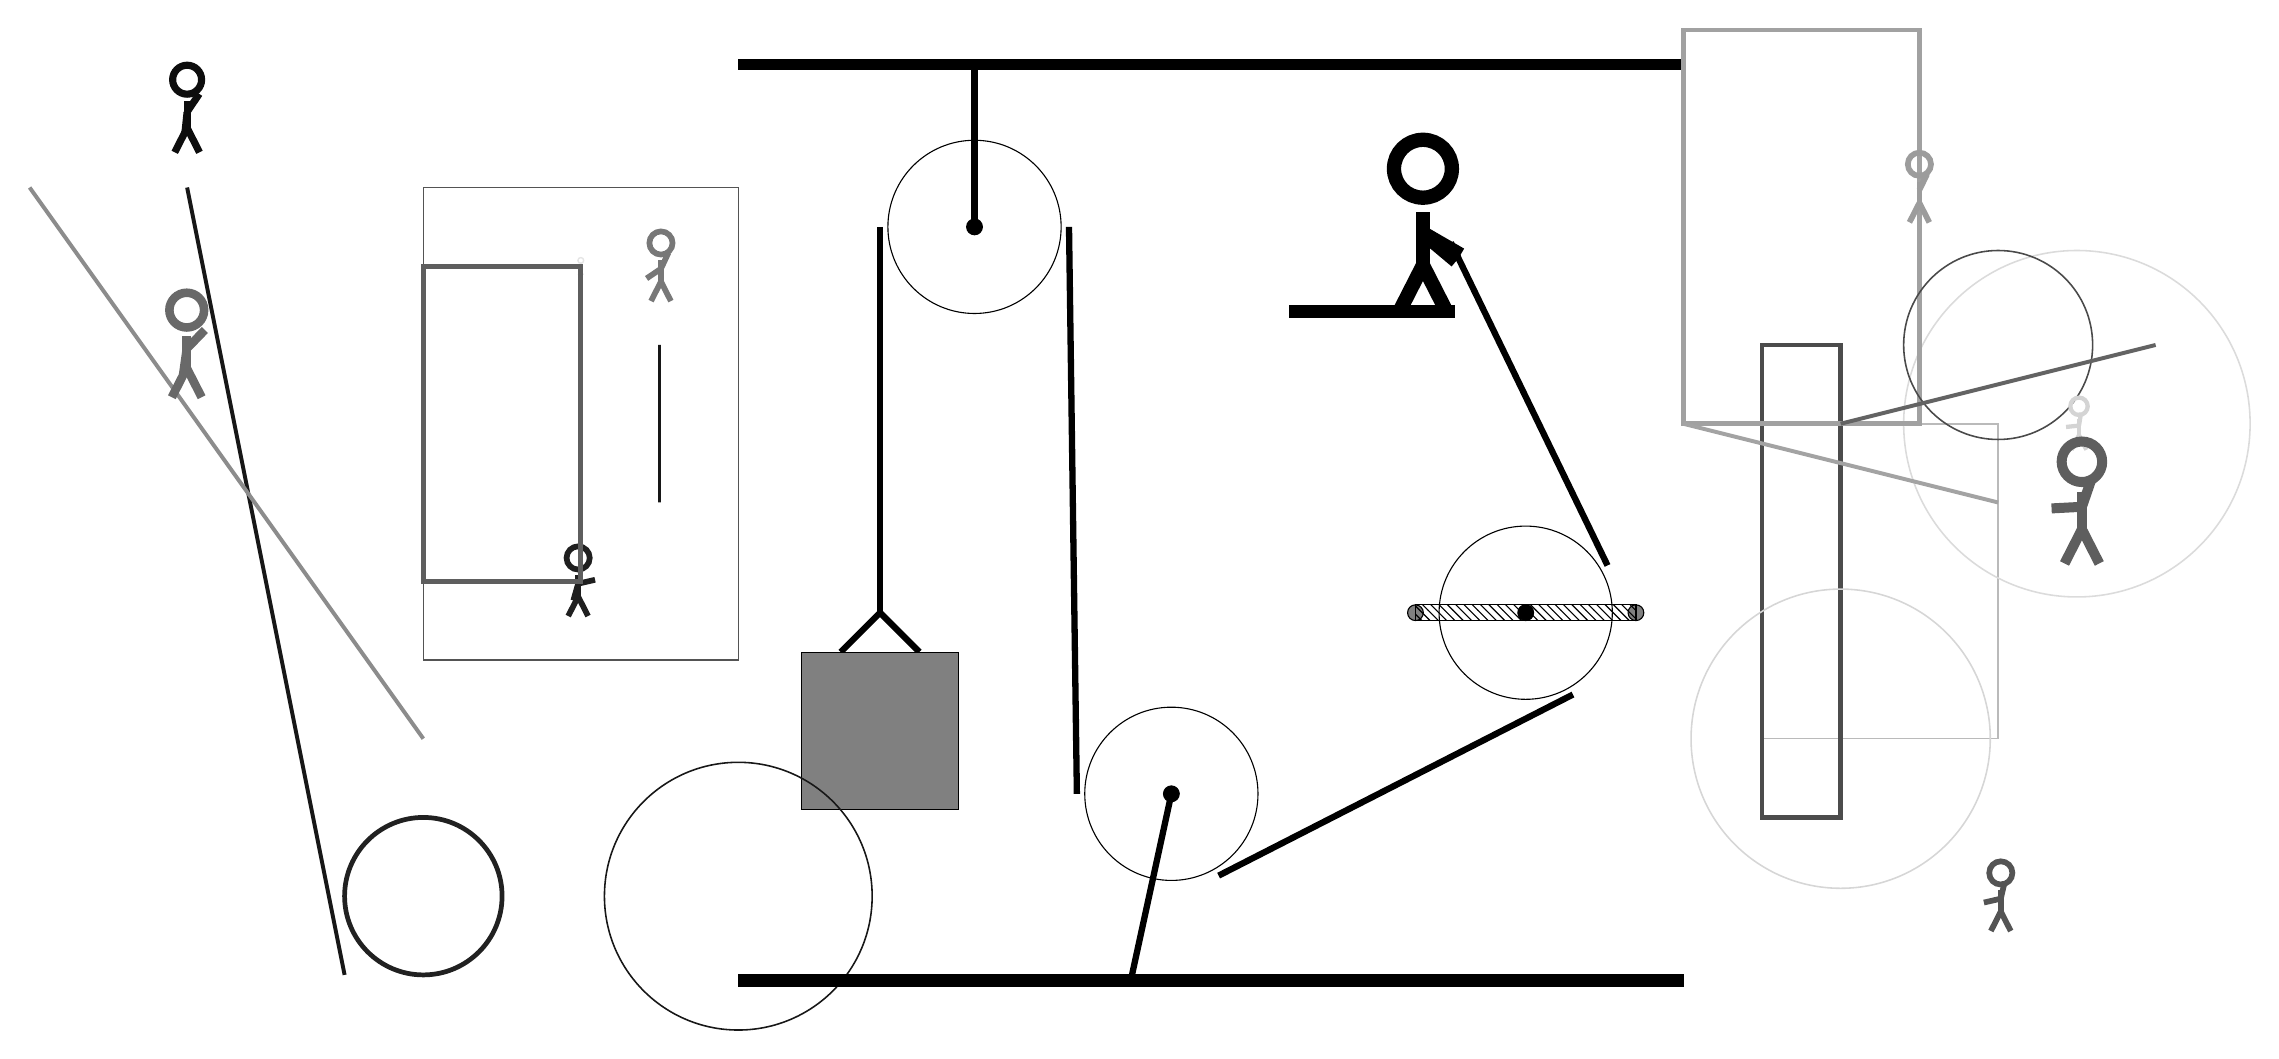
\begin{tikzpicture}
			%%%%% START %%%%%
			
			\draw[fill=black] (-2, 11.5) rectangle (10, 11.625);
			
			\draw (1, 9.5) circle (1.1);
			\draw[fill=black] (1, 9.5) circle (0.1);
			\draw[line width=0.8mm] (1, 11.5) -- (1, 9.5);
			
			\draw (3.5, 2.3) circle (1.1);
			\draw[fill=black] (3.5, 2.3) circle (0.1);
			\draw[line width=0.8mm] (3.5, 2.3) -- (3.0, 0);
			
			\draw[fill=white](8, 4.6) circle (1.1);
			\draw[fill=black] (8, 4.6) circle (0.1);
			\draw[fill=black!50] (9.4, 4.6) circle (0.1);
			\draw[fill=black!50] (6.6, 4.6) circle (0.1);
			\draw[pattern=north west lines, pattern color=black] (6.6, 4.7) rectangle (9.4, 4.5);
			
			\draw[line width=0.8mm](-0.7, 4.1) --  (-0.2, 4.6) -- (0.3, 4.1);
			\draw[fill=black!50] (-1.2, 4.1) rectangle (0.8, 2.1);
			
			\draw[line width=0.8mm](-0.2, 9.5) -- (-0.2, 4.6);
			\centerarc[line width=0.8mm](1, 9.5)(180:0:1.2000000000000002)
			\draw[line width=0.8mm](2.2, 9.5) -- (2.3, 2.3);
			\centerarc[line width=0.8mm](3.5, 2.3)(180:300:1.2000000000000002);
			\draw[line width=0.8mm](4.1, 1.2608) -- (8.6, 3.5608);
			\centerarc[line width=0.8mm](8, 4.6)(300:390:1.2000000000000002);
			\draw[line width=0.8mm](9.0392, 5.2) -- (7.05, 9.3);
			
			\node[line width=0.3mm, color=black!88] at (-4, 5) {\Strichmaxerl[4][74][13]};
			
			\draw[line width=0.6mm, color=black!34] (11, 12) rectangle (12, 12);
			\draw[line width=0.5mm, color=black!91](-7, 0) -- (-9, 10);
			\draw [line width=0.2mm, color=black!91](-2, 1) circle (1.7);
			\draw[line width=0.5mm, color=black!45](-6, 3) -- (-11, 10);
			
			\draw[line width=0.3mm, color=black!91] (-3, 8) rectangle (-3, 6);
			\draw[line width=0.2mm, color=black!27] (11, 7) rectangle (14, 3);
			\node[line width=0.2mm, color=black!10] at (-4, 9) {\Strichmaxerl[1][86][89]};
			\node[line width=0.3mm, color=black!67] at (14, 1) {\Strichmaxerl[4][13][77]};
			\draw [line width=0.2mm, color=black!14](15, 7) circle (2.2);
			\node[line width=0.2mm, color=black!53] at (-3, 9) {\Strichmaxerl[4][34][65]};
			\draw[line width=0.6mm, color=black!70] (11, 2) rectangle (12, 8);
			\node[line width=0.5mm, color=black!95] at (-9, 11) {\Strichmaxerl[5][84][56]};
			
			\node[line width=0.4mm, color=black!59] at (-9, 8) {\Strichmaxerl[6][82][46]};
			\draw[line width=0.6mm, color=black!37] (10, 7) rectangle (13, 12);
			\draw [line width=0.2mm, color=black!71](14, 8) circle (1.2);
			\draw [line width=0.2mm, color=black!16](12, 3) circle (1.9);
			\draw[line width=0.2mm, color=black!67] (-2, 4) rectangle (-6, 10);
			\node[line width=0.2mm, color=black!17] at (15, 7) {\Strichmaxerl[3][6][81]};
			
			\draw[line width=0.5mm, color=black!36](14, 6) -- (10, 7);
			\draw [line width=0.6mm, color=black!87](-6, 1) circle (1.0);
			
			\draw[line width=0.5mm, color=black!61](12, 7) -- (16, 8);
			\node[line width=0.3mm, color=black!63] at (15, 6) {\Strichmaxerl[7][3][71]};
			\draw[line width=0.6mm, color=black!63] (-4, 5) rectangle (-6, 9);
			\node[line width=0.5mm, color=black!39] at (13, 10) {\Strichmaxerl[4][90][64]};
			
			
			\node at (6.75, 9.5) {\Strichmaxerl[10][-220][-30]};
			\draw[fill=black] (5, 8.5) rectangle (7.1, 8.35);
			
			\draw[fill=black] (-2, 0) rectangle (10, -0.15);
			
			%%%%% END %%%%%
		\end{tikzpicture}
	\end{figure}	
\end{document}